%%%%%%%%%%%%%%%%%%%%%%%%%%%%%%%%%%%%%%%%%%%
%%% DOCUMENT PREAMBLE %%%
\documentclass[english, a4paper]{report}
\usepackage[T1]{fontenc}            % Riktig fontencoding
\usepackage[font=small,labelfont=bf]{caption} % Fin figur-undertekst
\usepackage{url}                    % Skrive url-er
\usepackage[english]{babel}           % Ordelingsregler, osv (velg språk her)
\usepackage[utf8]{inputenc}         % Riktig tegnsett
\usepackage{float}                  % Figurer dukker opp der du ber om
\usepackage{amsmath} 
\usepackage{graphicx}               % Inkludere bilder
\graphicspath{{images/}}
%\usepackage{listings}               % programeringskode
%\usepackage{minted}                 % for coding
%\usepackage{xcolor}                 % for coding

% ---------------------------------------------------------

% kapittelinndeling
\renewcommand{\thepart}{\arabic{part})}
\renewcommand\thesection{\arabic{section}}
\renewcommand{\thesubsection}{\alph{subsection})} % Alph = ABC, alph = abc
\renewcommand{\thesubsubsection}{\roman{subsubsection})}

% LaTeX symbol
\newcommand{\latex}{\LaTeX\xspace}

%---------------------------------------------------------
\pdfinfo{
%   /Title () 
	/Author (Henrik Løland Gjestang) 
	/Creator () 
	/Producer () 
	/Subject () 
	/Keywords () 
}
% ---------------------------------------------------------



%------------------------------------------------------------
% Forside
% ----------------------------------------------------------
\begin{document}
\begin{titlepage}
\begin{center}

\textsc{}\\[1.0cm]
\textsc{\Large Master essay}\\[0.5cm]
\rule{\linewidth}{0.5mm} \\[0.4cm]
{ \huge \bfseries A look on neural networks}\\[0.10cm]
\rule{\linewidth}{0.5mm} \\[1.5cm]
%\textsc{\Large oblig x}\\
%\medbreak
%\textsc{\Large henriklg}\\
\textsc{}\\[7.0cm]

% Av hvem?(kopier for flere personer, feks ved samarbeid)
\begin{minipage}{0.69\textwidth}
    \begin{center} \large
        Henrik Løland Gjestang\\ \url{henriklg@fys.uio.no} \\[0.8cm]
    \end{center}
\end{minipage}
\vfill

% Dato nederst
\large{Date: \today}
\end{center}
\end{titlepage}
% ----------------------------------------------------------

%%%%%%%%%%%%%%%%%%%%%%%%%%%%%%%%%%%%%%%%%%%%%%%%%%%%%%%%%%%%
\section*{Abstract}
%-----------------------------------------------------------
The abstract gives the reader a quick overview of what has been done and the most important results.


% ----------------------------------------------------------
\tableofcontents
\newpage
% ----------------------------------------------------------




%%%%%%%%%%%%%%%%%%%%%%%%%%%%%%%%%%%%%%%%%%%%%%%%%%%%%%%%%%%%
\section{Introduction}
%-----------------------------------------------------------
%Explain the aims and rationale for the physics case and what you have done. At the end of the introduction you should give a brief summary of the structure of the report. Motivate the reader and give overarching ideas. Describe what has been done and the structure of the report (how is it organized).

In this project, we aim to design and develop a system for analyzing medical videos from a camera pill, as seen in figure \ref{fig:pill-cam}. The pill is swallowed and records video of the entire digestive system and stores it on a onboard chip - the goal is to be able to detect different irregularities in the patients digestive system, like a colon polyp, Chron's disease, Colorectal cancer, etc. By using video object tracking, object detection, machine learning or other relevant tools or mechanisms.

Neural networks models that I would like to explore further for this purpose are Convolutional neural networks (CNN), Recurrent neural networks (RNN), Capsule neural networks, Long Short-Term memory networks and more.

The main idea is to go beyond image-based methods and also exploit the time factor of the data. 
The videos we will be using for this is delivered by Bærum Hospital, and is carefully labeled by professionals for use as training data for the neural networks. For simplicity, much or all of the training data is from regular "bottom-up" colonoscopy. And I will not go into much detail about the camera pill itself as this is a outside of the scope of this paper.

\begin{figure}[H]
\begin{center}
 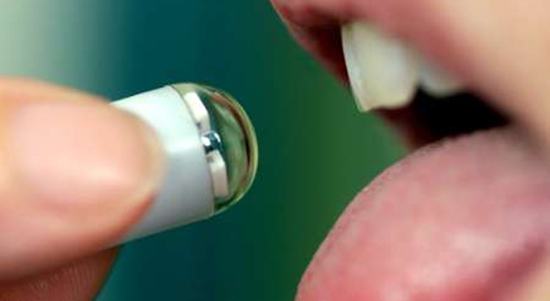
\includegraphics[width=\textwidth]{pill-cam.jpg}
 \caption{Illustration of how such a camera pill could look like. \cite{PillCamCameraPill}}
 \label{fig:pill-cam}
 \end{center}
\end{figure}

Colon cancer is the third most common cause of cancer mortality for both men and women \cite{jemalCancerStatistics20102010}, and it is a condition where early detection is of clear value for the ultimate survival of the patient. As statistics show that 15\% of male and female above 50 years are at risk (SOURCE), the procedure is recommended on a regular basis (every 3-5 years) for the population over 50, and from an earlier age for high-risk groups. Colonoscopy is a demanding procedure requiring an significant amount of time by specialized physicians, in addition to the discomfort and risks inherent in the procedure. Thus, traditional methods based on colonoscopy are not cost-effective for population-based screening purposes, so only about 2-3\% of the target population is reached at present. Moreover, the cost of a population screening program is prohibitively expensive. In the US, the colonoscopy is the most expensive cancer screening process with annual costs of \$10 billion dollars (\$1100 per person) (SOURCE). In Norway, we have similar costs of around \$1000 per person, with a time consumption of about 1 doctor-hour and 2 nurse-hours, per examination. By researching an automatic system for a camera pill, the aim is to greatly increase the number of patients that can be examined, i.e., making the public health care system more scalable and cost effective, while at the same time reducing the need for intrusive procedures like "bottom-up" examinations like colonoscopy.





%%%%%%%%%%%%%%%%%%%%%%%%%%%%%%%%%%%%%%%%%%%%%%%%%%%%%%%%%%%%
\section{Method}
%-----------------------------------------------------------
Theoretical models and technicalities. Describe how you implemented the methods and also say something about the structure and the algorithms used and central parts of code. Plug in some calculations to demonstrate your code, such as selected runs used to validate and verify results.




%%%%%%%%%%%%%%%%%%%%%%%%%%%%%%%%%%%%%%%%%%%%%%%%%%%%%%%%%%%%
\section{Results and discussion}
%-----------------------------------------------------------
Present the results. Give critical discussion of your work and place it in the correct context. Try to relate your work to other calculations/studies. The reader should be able to reproduce your calculations if they wanted to. Remember to explain all input variables. Make sure figures and tables contain enough information in their captions/labels/axis so that the reader can gain a first impression of your work.




%%%%%%%%%%%%%%%%%%%%%%%%%%%%%%%%%%%%%%%%%%%%%%%%%%%%%%%%%%%%
\section{Conclusions and perspectives}
%-----------------------------------------------------------
State your main findings and interpretations. Try as far as possible to present perspectives for future work. Discuss the pros and cons of the methods and possible improvements.
\cite{russellArtificialIntelligenceModern2016}


\newpage
\bibliography{../references}
\bibliographystyle{ieeetr}

\end{document}